\documentclass[14pt]{extbook}
\usepackage{multicol, enumerate, enumitem, hyperref, color, soul, setspace, parskip, fancyhdr} %General Packages
\usepackage{amssymb, amsthm, amsmath, latexsym, units, mathtools} %Math Packages
\everymath{\displaystyle} %All math in Display Style
% Packages with additional options
\usepackage[headsep=0.5cm,headheight=12pt, left=1 in,right= 1 in,top= 1 in,bottom= 1 in]{geometry}
\usepackage[usenames,dvipsnames]{xcolor}
\usepackage{dashrule}  % Package to use the command below to create lines between items
\newcommand{\litem}[1]{\item#1\hspace*{-1cm}\rule{\textwidth}{0.4pt}}
\pagestyle{fancy}
\lhead{Progress Quiz 10}
\chead{}
\rhead{Version B}
\lfoot{1995-1928}
\cfoot{}
\rfoot{test}
\begin{document}

\begin{enumerate}
\litem{
Solve the equation below. Then, choose the interval that contains the solution.\[ -18(-7x + 19) = -8(-10x -13) \]\begin{enumerate}[label=\Alph*.]
\item \( x \in [-1.84, 2.16] \)
\item \( x \in [7.7, 13.7] \)
\item \( x \in [3.17, 6.17] \)
\item \( x \in [-8.17, -1.17] \)
\item \( \text{There are no real solutions.} \)

\end{enumerate} }
\litem{
Solve the linear equation below. Then, choose the interval that contains the solution.\[ \frac{4x + 7}{3} - \frac{-5x + 3}{7} = \frac{3x -6}{2} \]\begin{enumerate}[label=\Alph*.]
\item \( x \in [-3, 0.1] \)
\item \( x \in [-19.9, -17.2] \)
\item \( x \in [-11, -9.4] \)
\item \( x \in [-10.5, -8.7] \)
\item \( \text{There are no real solutions.} \)

\end{enumerate} }
\litem{
Find the equation of the line described below. Write the linear equation as $ y=mx+b $ and choose the intervals that contain $m$ and $b$.\[ \text{Parallel to } 5 x + 4 y = 3 \text{ and passing through the point } (8, 6). \]\begin{enumerate}[label=\Alph*.]
\item \( m \in [-1.74, -0.87] \hspace*{3mm} b \in [-16.1, -14.6] \)
\item \( m \in [-1.74, -0.87] \hspace*{3mm} b \in [13.5, 16.4] \)
\item \( m \in [-1.02, -0.79] \hspace*{3mm} b \in [13.5, 16.4] \)
\item \( m \in [-1.74, -0.87] \hspace*{3mm} b \in [-2.1, -1.7] \)
\item \( m \in [0.81, 1.59] \hspace*{3mm} b \in [-4.3, -2.9] \)

\end{enumerate} }
\litem{
First, find the equation of the line containing the two points below. Then, write the equation as $ y=mx+b $ and choose the intervals that contain $m$ and $b$.\[ (-11, 6) \text{ and } (-7, 3) \]\begin{enumerate}[label=\Alph*.]
\item \( m \in [-3.8, -0.7] \hspace*{3mm} b \in [-3.6, -2] \)
\item \( m \in [-3.8, -0.7] \hspace*{3mm} b \in [0.1, 3.7] \)
\item \( m \in [-3.8, -0.7] \hspace*{3mm} b \in [15.6, 17.9] \)
\item \( m \in [-3.8, -0.7] \hspace*{3mm} b \in [8.4, 11.7] \)
\item \( m \in [0.1, 1.4] \hspace*{3mm} b \in [7.9, 9.2] \)

\end{enumerate} }
\litem{
First, find the equation of the line containing the two points below. Then, write the equation as $ y=mx+b $ and choose the intervals that contain $m$ and $b$.\[ (2, 6) \text{ and } (10, 2) \]\begin{enumerate}[label=\Alph*.]
\item \( m \in [-1.43, 0.27] \hspace*{3mm} b \in [2.61, 4.6] \)
\item \( m \in [-1.43, 0.27] \hspace*{3mm} b \in [5.88, 8.39] \)
\item \( m \in [-1.43, 0.27] \hspace*{3mm} b \in [-7.53, -6.79] \)
\item \( m \in [-1.43, 0.27] \hspace*{3mm} b \in [-8.5, -7.99] \)
\item \( m \in [-0.34, 1.24] \hspace*{3mm} b \in [-3.44, -2.64] \)

\end{enumerate} }
\litem{
Write the equation of the line in the graph below in Standard form $Ax+By=C$. Then, choose the intervals that contain $A, B, \text{ and } C$.
\begin{center}
    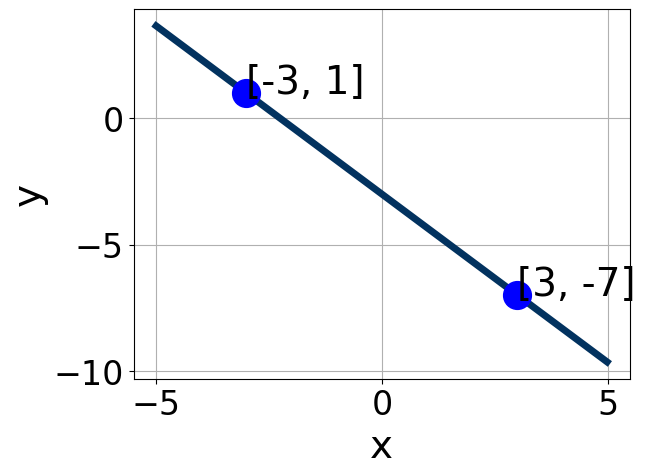
\includegraphics[width=0.5\textwidth]{../Figures/linearGraphToStandardB.png}
\end{center}
\begin{enumerate}[label=\Alph*.]
\item \( A \in [1.4, 4.7], \hspace{3mm} B \in [-2.24, -1.31], \text{ and } \hspace{3mm} C \in [2.8, 4.3] \)
\item \( A \in [-2.5, 1.3], \hspace{3mm} B \in [-1.97, -0.96], \text{ and } \hspace{3mm} C \in [-0.7, 2.6] \)
\item \( A \in [-2.5, 1.3], \hspace{3mm} B \in [0.68, 1.32], \text{ and } \hspace{3mm} C \in [-3.2, 0.1] \)
\item \( A \in [1.4, 4.7], \hspace{3mm} B \in [1.75, 2.41], \text{ and } \hspace{3mm} C \in [-5, -3.6] \)
\item \( A \in [-5.3, -2.8], \hspace{3mm} B \in [1.75, 2.41], \text{ and } \hspace{3mm} C \in [-5, -3.6] \)

\end{enumerate} }
\litem{
Solve the linear equation below. Then, choose the interval that contains the solution.\[ \frac{5x + 6}{6} - \frac{-6x -4}{5} = \frac{5x -4}{3} \]\begin{enumerate}[label=\Alph*.]
\item \( x \in [-8.55, -5.55] \)
\item \( x \in [-6.18, -3.18] \)
\item \( x \in [-42.18, -35.18] \)
\item \( x \in [-2.52, 0.48] \)
\item \( \text{There are no real solutions.} \)

\end{enumerate} }
\litem{
Write the equation of the line in the graph below in Standard form $Ax+By=C$. Then, choose the intervals that contain $A, B, \text{ and } C$.
\begin{center}
    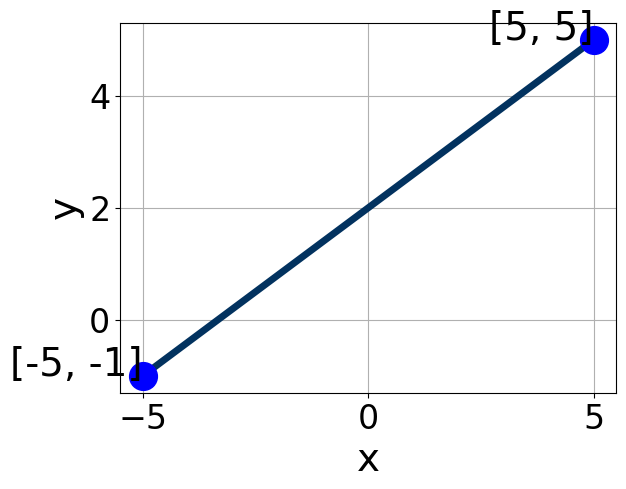
\includegraphics[width=0.5\textwidth]{../Figures/linearGraphToStandardCopyB.png}
\end{center}
\begin{enumerate}[label=\Alph*.]
\item \( A \in [-4.75, 2.25], \hspace{3mm} B \in [0.95, 1.15], \text{ and } \hspace{3mm} C \in [3, 6] \)
\item \( A \in [3, 8], \hspace{3mm} B \in [3.92, 5.71], \text{ and } \hspace{3mm} C \in [7, 18] \)
\item \( A \in [-9, -4], \hspace{3mm} B \in [-4.73, -3.12], \text{ and } \hspace{3mm} C \in [-15, -6] \)
\item \( A \in [3, 8], \hspace{3mm} B \in [-4.73, -3.12], \text{ and } \hspace{3mm} C \in [-15, -6] \)
\item \( A \in [-4.75, 2.25], \hspace{3mm} B \in [-1.46, -0.73], \text{ and } \hspace{3mm} C \in [-6, 0] \)

\end{enumerate} }
\litem{
Find the equation of the line described below. Write the linear equation as $ y=mx+b $ and choose the intervals that contain $m$ and $b$.\[ \text{Perpendicular to } 9 x - 8 y = 8 \text{ and passing through the point } (9, 8). \]\begin{enumerate}[label=\Alph*.]
\item \( m \in [-0.89, -0.73] \hspace*{3mm} b \in [12.5, 16.5] \)
\item \( m \in [-0.89, -0.73] \hspace*{3mm} b \in [-16.5, -14.2] \)
\item \( m \in [-1.33, -1.12] \hspace*{3mm} b \in [12.5, 16.5] \)
\item \( m \in [0.82, 1.01] \hspace*{3mm} b \in [-0.3, 0.1] \)
\item \( m \in [-0.89, -0.73] \hspace*{3mm} b \in [-1.3, -0.5] \)

\end{enumerate} }
\litem{
Solve the equation below. Then, choose the interval that contains the solution.\[ -19(-3x + 16) = -8(-9x + 17) \]\begin{enumerate}[label=\Alph*.]
\item \( x \in [-12.2, -8.2] \)
\item \( x \in [-30.33, -28.33] \)
\item \( x \in [1.41, 4.41] \)
\item \( x \in [27.33, 32.33] \)
\item \( \text{There are no real solutions.} \)

\end{enumerate} }
\end{enumerate}

\end{document}